%%%%%%%%%%%%%%%%%%%%%%%%%%%%%%%%%%%%%%%%%%%%%%%%%%%%%%%%%%%%%%%%%%%%%%%%%%%%%%%
% Overview of the methodology to be used.
% \newpage

\begin{figure}
    \centering
    \graphicspath{ {../schemas/methodology/} }
    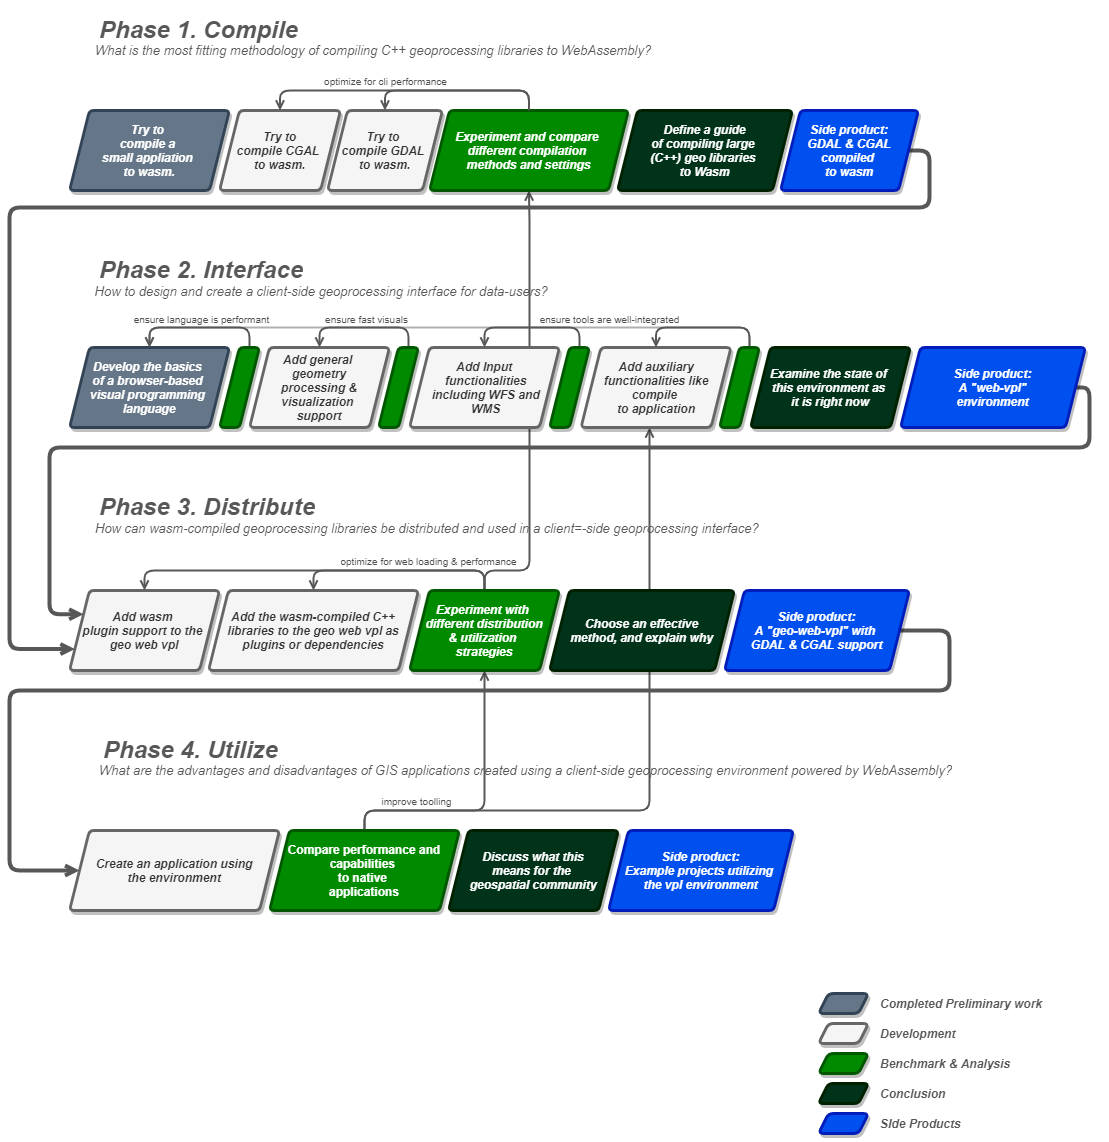
\includegraphics[width=14cm]{method.png}
    \caption{Methodology schema}
    \label{fig:method}
\end{figure}

\section{Methodology}

To find answers to the research questions posed, many different aspects of client-side web technology will have to be studied, and sizable, complex software will have to be written. Moreover, these aspects and the software are all interlinked and interdependent.

This chapter covers the methodology posed to untangle this, and the choices made to eventually create this method. \reffig{fig:method} overs an overview. As shown, this study will be divided into four phases, matching the four sub-research questions. Every phase will cover two goals. The primary goal is to answer its corresponding research question, and to cover the process towards this answer. The secondary goal is to describe the development of the software required to form this answer. This software can be seen as a "side product", and will be a required starting point to answer subsequent questions. 

% 1. Compile, 2. Interface, 3. Synthesize, and 4. Utilize.

Every phase contains a number of development \& analysis steps. The reasoning behind these steps are covered by the following sub-chapters.  

The methodology used can be characterized as both incremental and iterative. Its incremental nature means that every phase, and every step within a phase, will produce meaningful in-between products \& results. This ensures the study will be insightful, even in the case the full scope of this study might become unfeasible. It is also vital for making the methodology iterative. 

The study's iterative nature, represented by the cyclic paths within \reffig{fig:method}, means that analysis and benchmarks will not be postponed until the end of the study, and will instead be carried out during each step. This makes sure obstacles are discovered early, and the trajectory of the study can be adjusted dynamically.  

This is important to restate. The schema acts as a general guide, and is subject to change, based on the obstacles encountered during the study. Also, as \reffig{fig:method} suggests, Phase 1 and 2 can be executed in parallel, and require no particular order. 

%%%%%%%%%%%%%%%%%%%%%%%%%%%%%%%%%%%%%%%%%%%%%%%%%%%%%%%%%%%%%%%%%%%%%%%%%%%%%%%

\subsection{Phase 1: Compile}

% not as easy 
The first phase will be about the procedure to successfully compile C++ geoprocessing libraries to WebAssembly. This might not be as easy as using normal C++ compilers, based on the experience gained by preliminary work (SOURCE: CITYJSON CHECKER). WebAssembly is containerized and platform independent, making aspects such as an SDK, sub-dependencies called using environment variables, and IO (file reading and writing) possible obstacles. These aspects might be solved by using or writing wrapper libraries and using file system workarounds. 

% question & steps to answer
This is why an entire research question is dedicated to finding an answer to this problem: \textbf{"What is the most fitting methodology of compiling C++ geoprocessing libraries to WebAssembly?"}. 'Fitting' in this context refers to the specific requirements posed by geoprocessing libraries. The libraries are complex and sizable, and the geodata used as input even more so. This means special attention will be given to these aspects. Standard compiler effectiveness criteria, such as portability (smallest file size), and performance, will also be considerations during the assessment of methodologies.  

While the question poses to find the \textit{best} compilation method, if it turns out that only one method makes it possible to compile sizable geo-libraries, this phase will nonetheless regard itself as successful. The question will have to be rephrased in that case. 

% performance
\subsubsection*{Performance}
The performance benefit of WebAssembly is an important component of why WebAssembly might be beneficial for client-side geoprocessing. As such, this phase is interested in confirming whether this is the case for geoprocessing applications. Once a sufficient compilation method is found, individual functions of geoprocessing libraries will be benchmarked using three different methods: 

\begin{itemize}
    \item Compiled and run as native binary (g++), 
    \item Compiled to wasm, run natively (WASI),
    \item Compiled to asm.js, run natively (NODE.js),
\end{itemize}

% why cgal & GDAL
\subsubsection*{Test Cases}
CGAL \& GDAL will be used as examples of "C++ geoprocessing libraries" for this phase. For one, these libraries are well established and relevant to geoprocessing as a whole. Many other geo-libraries depend on them. Moreover, they are properly sizable and complex, making it highly likely the problems described earlier will be encountered. We could choose "easier" libraries, but this will not be representative of most C++ geoprocessing libraries. And, while CGAL, and GDAL will be this phase's primary subject, the answer of this research question aims to be a guide applicable to all geoprocessing libraries. 

%%%%%%%%%%%%%%%%%%%%%%%%%%%%%%%%%%%%%%%%%%%%%%%%%%%%%%%%%%%%%%%%%%%%%%%%%%%%%%%

\subsection{Phase 2: Interface}

The possibility of geodata processing in a web application seriously transforms its nature. Because of this, it is important to consider how the user interface of said applications will have to change in order to facilitate geodata processing. 
Phase two seeks and answer to this with the research question: \textit{How to design and create a client-side geoprocessing interface?}. 

This question can be split in two. A: \textit{What is a desired interface for geoprocessing?} and B:  \textit{How can client-side web technologies facilitate this interface?}. 

% WHY vpl
\subsubsection*{A: VPL}
Finding a definitive answer for question A is an endeavour so large that it is beyond the scope of this study. Instead, this study will make an informed assumption, and start its reasoning from there. 
User experience studies (SOURCE), preliminary experiments (SOURCE) and interviews (SOURCE), have culminated to the choice of designing a Visual Programming Language(VPL) to act as a geoprocessing interface. This has several reasons behind it.



Web -> Sharable -> User friendly -> increase reach of geodata processing
Debuggable- > visualizing in-between steps. rendering, caching, experimenting
Geodata processing -> It is often the drawing people make when explaining geodata pipelines

This study will include implementation details of the VPL, and the design considerations made during its development. These decisions will be informed by analysis of exsting geo-vpl's, and studies discussing the usability aspects of VPL's (SOURCE: VPL Usability paper,  Ravi Peter)


\subsubsection*{B: VPL}

Now the question, how to get there from a browser?
- no vpl's exist yet, so have to be developed from scratch
- What features from HTML / CSS / JS can we utilize to get there

- go over all extra features you described earlier, like the need to be compiled to an app, 
- etc. etc. etc.

What makes a GIS VPL different from just any VPL???? 

The tool and can be additionally used for acquiring, visualizing, and saving geodata.


This phase seeks to answer this question in a practical manner, by creating this interface / environment.


% \subsubsection*{Conclusions and Discussion on using a web based VPL for geo-processing}

% Additionally, this study will give an answer to if and how a VPL contributed to more usable geoprocessing. This will be a purely qualitative assessment, based on the findings and experience using the environment.  


% The current plan is to shape this like a visual programming language. 

Just like the entire project, the development trajectory during phase 2 will be done incrementally, ensuring results can be produced and shown during all steps of the development. 




\subsubsection*{Detais}


Creating a client-side geoprocessing application comes with many specific design considerations. 



(mention preliminary work)

- 2D Canvas API / SVG 

- DAG : Directed Acyclic Graph

- Granular classes 


\subsubsection*{Go over all steps}


basic mathematical and geometry procedures. 

and will not contain any geodata processing capabilities, nor WebAssembly. 

Write down MOSCOW






%%%%%%%%%%%%%%%%%%%%%%%%%%%%%%%%%%%%%%%%%%%%%%%%%%%%%%%%%%%%%%%%%%%%%%%%%%%%%%%
\subsection{Phase 3: Distribute}

% performant and sharable geoprocessing
% portability


The third phase is characterized by distribution. 
This phase will test if using WebAssembly will indeed make geodata processing more portable.  
The research question goes: \textit{What is the best way of distributing wasm-compiled geoprocessing libraries, in order to use them within a client-side geoprocessing interface?}. 
This phase can be seen as a continuation of phase 1, but where the compilation research of phase 1 limits itself to native, CLI usage of WebAssembly, this phase introduces the web, and the developed interface during phase 2 as new factors to this research. Given this as the desired way of processing geodata, how can WebAssembly facilitate these desires? 

This will result in new benchmarks, and new analyses, now including factors like client-side (down)load times, compilation, and utilization. Answers will have to be given to questions such as \textit{Where do the wasm-compiled libraries live?} and \textit{ how are they cached? }.

One of the hypothetical obstacles during this phase is that an entire geoprocessing libraries will have to be downloaded, even if the user desires only a single function. A solution to this problem is to increase granularity, and split up the C++ libraries to several smaller ones, maybe even one wasm binary per function or class. This would be accompanied by WebAssemblies ability to accept dependencies at the time it is loaded into memory. 




%%%%%%%%%%%%%%%%%%%%%%%%%%%%%%%%%%%%%%%%%%%%%%%%%%%%%%%%%%%%%%%%%%%%%%%%%%%%%%%
\subsection{Phase 4: Utilize}

Finally, When the VPL contains all tools necessary to be used to properly process geodata, a final assessment can be made by using the environment to serve as an application. this assessment will try to answer: \textit{What are the advantages and disadvantages of GIS applications created using a client-side geoprocessing environment powered by WebAssembly?}. This question requires a native but comparable GIS application to test this against.  


I hypothesize that applications equipped with client-side geoprocessing open up a whole range of new possibilities for both academic \& commercial benefits. 
I intent to discuss these aspects of the study during this phase. 


% Three different 
% and these same applications will be created using the prototype web-VPL. 
% These two methods will then be compared on usability aspects and performance.   

% ## 5.3 Case Study

\subsubsection*{Case Study}

\begin{lstlisting}
# Demo Application: On Demand Triangulator + Isocurves

# Input: 
- Point Cloud

# Output
- Line Curves / .png render of line curves

# Steps: 
- Load ahn3 point-cloud 
  (WFS Input Widget | WFS Preview Widget)
- Visualize point cloud on top of base map of the netherlands 
  (WMS Input Widget | WMS > Preview Widget)
- Only select terrain points (list filter Operation)
- Construct a 2d polygon by clicking points on a map 
  (Polygon Input Widget)
- Select Area of interest using a 2d polygon 
  (Boundary Include Operation)
- Triangulate point cloud with a certain resolution 
  (Triangulate Operation)
- Intersect the mesh surface with a series of planes 
  (Isocurves from Mesh Operation)
- Preview data 
  (MultiLine Preview Widget)
- Export data 
  (MultiLine export Widget)
\end{lstlisting}
